\lab{Algorithm}{Change of Basis}{Change of Basis}
\label{lab:ChangeBasis}

\objective{Understand how to change the basis of a set of points.}

TODO: revise

\section*{Basis}

A basis for a vector space is a set of vectors such that every vector in the space can be expressed uniquely as a linear combination of the basis vectors.
In this lab we will take the coordinates in 2-d space and do various affine transformations.
For all these exercises we will use the points

\begin{lstlisting}
x = np.array([-1.5,-1.,-.5,0.,.5,1.,1.5,.75,-.75],[0.,-1.,-2.,-2.,-2.,-1.,0.,2.,2.]).T
\end{lstlisting}
A linear transformation can be thought of, conceptually, as changing our representation of the vectors of a space from one basis to another.
A change of basis is really just a linear transformation.
In a finite dimensional normed vector spaces like $\mathbb{R}^n$ a linear transformation, or a change of basis can be represented as a matrix.
The matrix maps any vector from the original space to its image under the linear transformation by left matrix multiplication.
In other words, any linear transformation $T : \mathbb{R}^n \to \mathbb{R}^n$ is linear if and only if there exists an $n\times n$ matrix $A$ such that $T\left(x\right) = A x$.
Let A be the matrix of points and x is the matrix that will perform the linear transformation.
So $A x$ will be the set of points in the new basis.

Different sorts of linear transformations can be represented by different types of matrices.

\section*{stretch}
To stretch a set of points, $A$ will be a diagonal matrix where the value in each position is the stretch in that direction.

\begin{figure}[H]
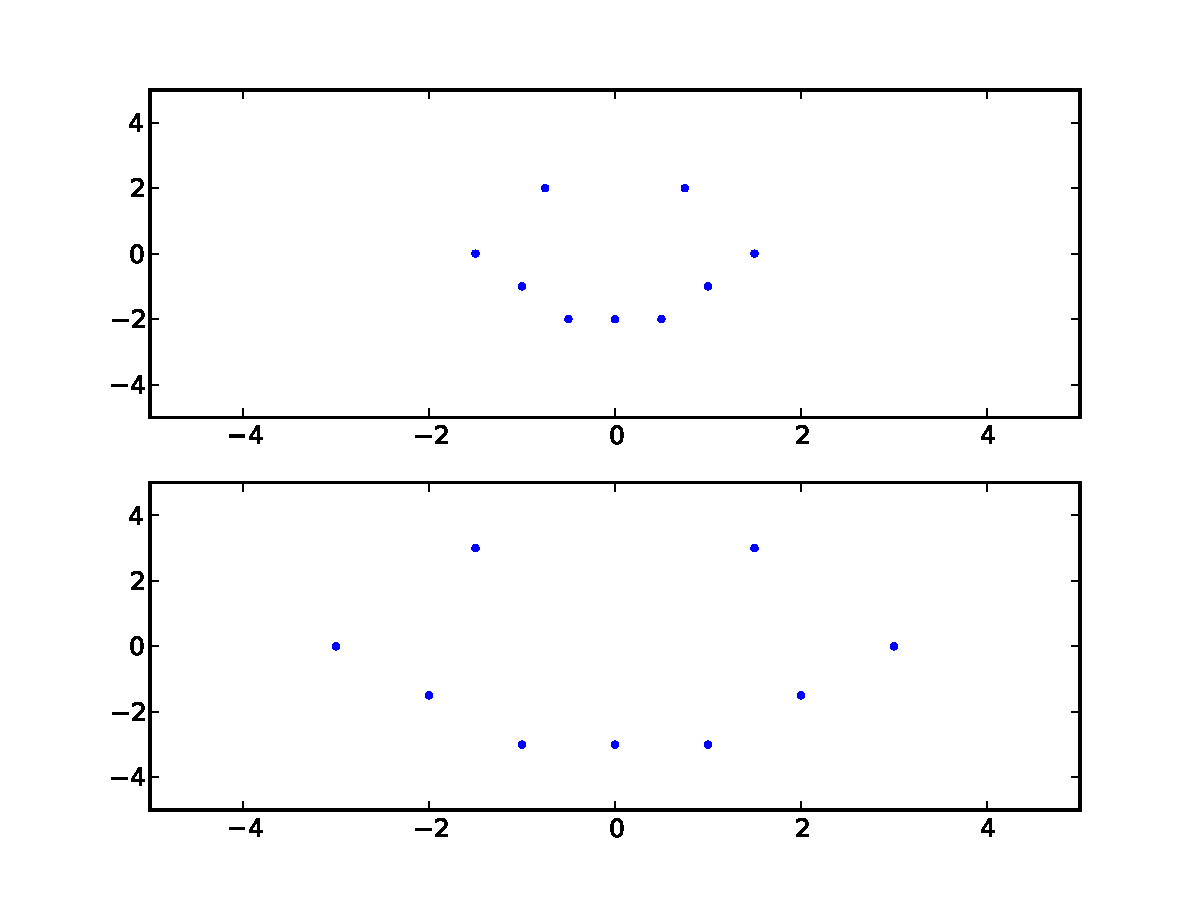
\includegraphics[scale = .5]{strench.pdf}
\caption{
An example of a stretch.
The top image is the original and the bottom is the modified image.
The streach was 2 in the x direction and 1.5 in the y direction.}
\end{figure}

\begin{problem}
Write a function that will accepts an array of points and how much to stretch them in each direction.
Plot the transformed points.
This can be done with the following code:
\begin{lstlisting}
import numpy as np
# now construct an array 'pts' with
# x values along its first column and
# y values along its second column
from matplotlib import pyplot as plt
plt.scatter(pts[:,0], pts[:,1])
plt.show()
\end{lstlisting}
\end{problem}

\section*{Rotation}
To do a rotation clockwise a set of points in angle $\theta$ (where $\theta$ is in radians) let
\[
M = \begin{pmatrix}
\cos(\theta) & -\sin(\theta) \\
\sin(\theta) & \cos(\theta) 
\end{pmatrix}
\]

\begin{figure}[H]
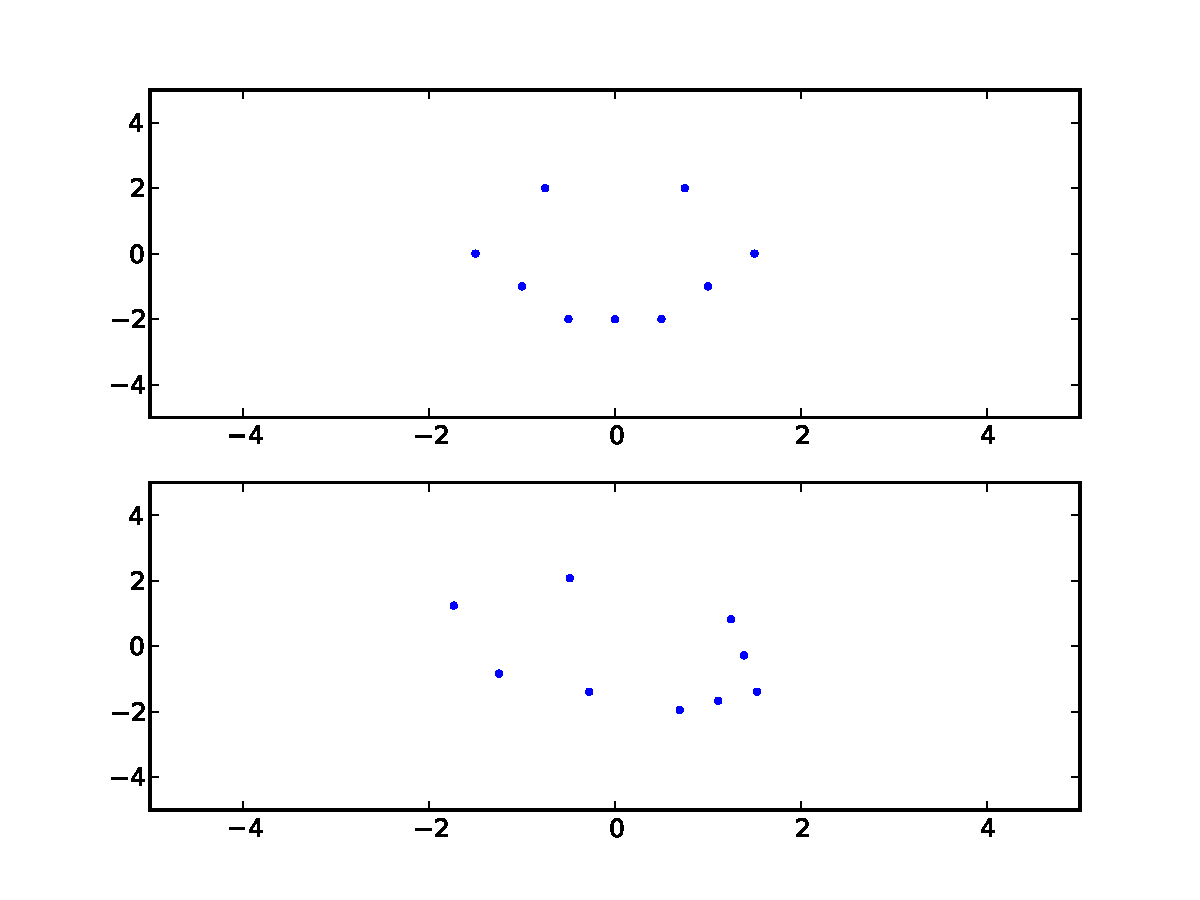
\includegraphics[scale = .5]{rotate.pdf}
\caption{
An example of a rotation.
The top image is the original and the bottom is the modified image.
The rotation angle was $\frac{3\pi}{16}$.}
\end{figure}

\begin{problem}
Write a function that will accept an array of points and how many radians to rotate the points.
Have it return a rotated version of the array of points.
Plot the transformed points.
\end{problem}

\section*{Shift}

Shifts are not linear transformations, but they can be performed easily with array operations.
They are a part of a broader class of transformations called ``affine transformations."
These are transformations of the form $T: \mathbb{R}^n \to \mathbb{R}^n$, $T(x) = A x + b$ where $A$ is an $n\times n$ matrix and $b \in \mathbb{R}^n$.
Affine transformations include all compositions of stretches, rotations, and shifts.

Let $b$ be a vector that represents shift that you add to $x$.
In order to shift a set of points, you add to the row how much you would like it to shift it in that direction, so to shift the set of points up by 2, \li{L = np.array([[0,2]])}.
You can use array broadcasting to do this.

\begin{figure}[H]
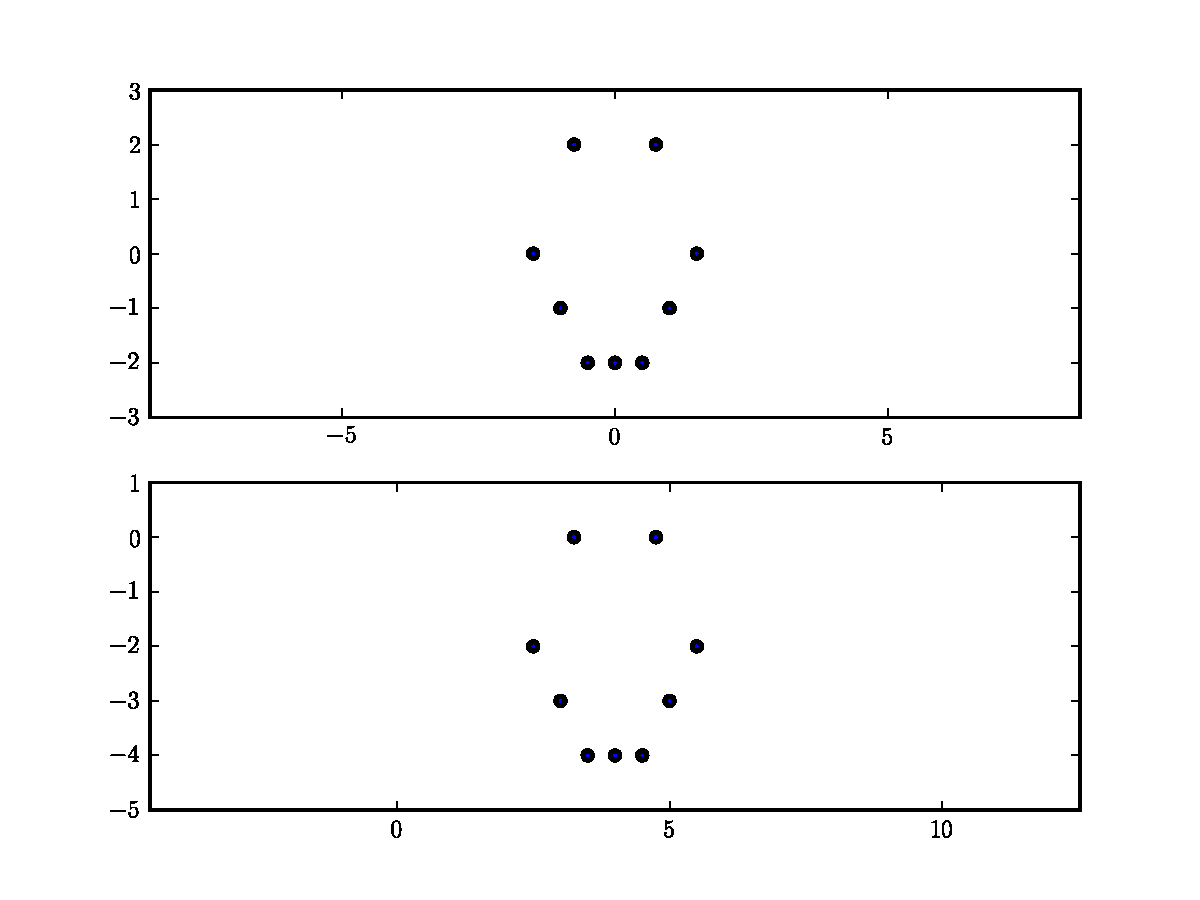
\includegraphics[scale = .5]{shift.pdf}
\caption{
An example of a shift.
The top image is the original and the bottom is the modified image.
The shift was 2 in the x direction and 1 in the y direction.}
\end{figure}

\begin{problem}
Write a function that will accept an array of points and how much to shift them in each direction.
Have the function plot the transformed points.
\end{problem}

\section*{Combination}
These transformations can be applied and combined into single affine transformations through function composition.
For example, if you want to apply a stretch, then rotate an array of points $x$, you can represent the stretch as a matrix $S$ and the rotation as a matrix $R$ and represent the combined transformation as $R S$.
The image of $x$ under both transformations will be $R S x$.
An example like this is shown in Figure \ref{basis:combo}.

\begin{figure}[H]
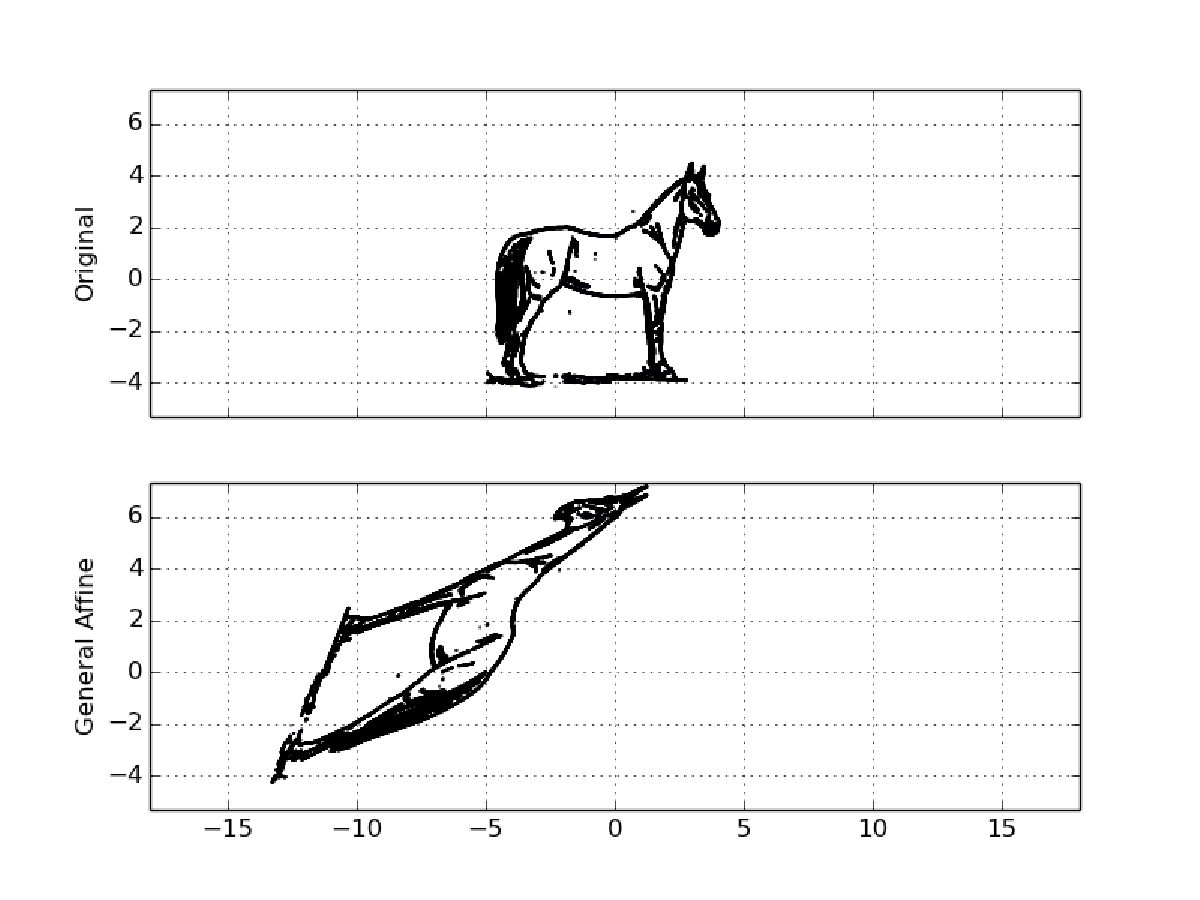
\includegraphics[scale = .5]{combo.pdf}
\caption{
A combination of linear transformations.
The stretch was 2 in each direction.
The rotation angle was $\frac{3\pi}{4}$.
The shift was 1 in the x direction and -2 in the y direction.}
\label{basis:combo}
\end{figure}

\begin{problem}
Write a function that will accepts a matrix of points and stretch, rotate and shift them.
\end{problem}

\section*{Images}

An Image is a 3d array where the first two dimensions are the location and the 3rd dimension is the RGB content.
To apply the above transformations one would need to move the position of the RGB arrays to match where the new transformation would have them.

\begin{figure}[H]

\includegraphics[scale = 2.0]{dream.png}
\caption{The original image}
\end{figure}

\begin{figure}[H]
\includegraphics[scale = .5]{rotateimg.pdf}
\caption{Rotated at an angle of $\frac{\pi}{4}$}
\end{figure}

TODO: clarify how to plot this.

\begin{problem}
Write a function that will accepts an image and how many radians to rotate the image.
The function will rotate the image around the center of the image and then show the rotated image.
HINTS: Make an array of ones that is $1.5$ times greater than the max of the height and width of the original image.
Change the x,y coordinates in the original image so the center is $(0,0)$.
Rotate the image and then center the image.
You might need to use for loops.
Allow your test cases to be small images.
\end{problem}


